\documentclass[menu.tex]{subfiles}
\graphicspath{ {images/} }
\begin{document}    
    \begin{tabular} {p{3.5cm} p{4cm} p{9cm}}
        \multicolumn{3}{c}{\begin{LARGE}Menú Semanal 3\end{LARGE}}\\
        \hline
    
        %---LUNES---%
        \pbox{20cm}
        {
            \rule{0pt}{3ex}\begin{large}\textbf{Lunes}\end{large}\\ 
            \rule{0pt}{2ex}Silpancho \\
            \includegraphics[scale=0.25]{Silpancho} 
        } & 
        \vspace{-1.8cm}
        \begin{compactitem} 
            \begin{footnotesize}
                \item Carne blanda sin grasa ni nervios en filetes
                \item 1 taza de arroz graneado cocido
                \item 4 papas medianas cocidas
                \item 4 huevos
                \item Tomate, Cebolla y Locoto
                \item Tomate, Cebolla y Locoto
                \item Pan molido cantidad suficiente
                \item Vinagre, Aceite
                \item Sal y Pimienta
            \end{footnotesize}
        \end{compactitem}&
        \vspace{-1.8cm}
        1. Sazonar la carne con sal y pimienta y adelgazar con el pan molido hasta que quede como un asado grande y delgado, se debe agregar pan molido constantemente y suficiente para que la carne no se rompa con los golpes. 
        2. Freír las papas previamente cocidas y cortadas en rodajas, los huevos y la carne apanada.
        3. Picar el tomate, la cebolla y el locoto en cuadritos chicos; mezclar y sazonar con sal, pimienta y vinagre.
        4. Servir en un plato poniendo una cama de arroz, distribuir unas cuantas papas, encima poner la carne, el huevo frito y decorar con la salsa cruda. \\
        \hline
        
        %---MARTES---%
        \pbox{20cm}
        {
            \rule{0pt}{3ex}\begin{large}\textbf{Martes}\end{large}\\ 
            \rule{0pt}{2ex}Sopa de maní \\
            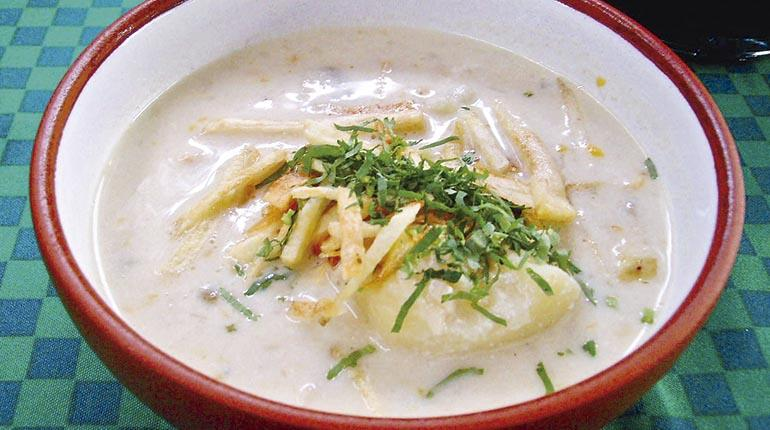
\includegraphics[scale=0.2]{sopa_de_mani} 
        } & 
        \vspace{-1.6cm}
        \begin{compactitem} 
            \begin{footnotesize}
                \item 6 nudos de carne de cordero  o costilla de vaca
                \item 1 cuchara de sal molida
                \item 6 papas
                \item \nicefrac{1}{2} taza de arvejas
                \item 1/2 taza de habas verdes
                \item 1 taza de maní molido
                \item 3 litros de agua para cocer la carne
                \item 1 taza de cebolla
                \item \nicefrac{1}{2} taza de tomate
                \item 1 cucharilla de comino
                \item 2 dientes de ajo
                \item 1 cuchara de orégano
                \item 1 cuchara de perejil
                \item 1 \nicefrac{1}{2} cuchara de ají  amarillo molido
                \item \nicefrac{1}{4} taza de aceite
            \end{footnotesize}
        \end{compactitem}&
        \vspace{-1.6cm}
        Parta las papas peladas en cuatro, pele las arvejas, pique la cebolla menuda y el tomate pelado. Fría la cebolla en el aceite. En una olla ponga al fuego los 3 litros de agua. Antes que empiece a hervir, agréguele la carne. Deje dar un hervor y ponga la sal, el tomate, la cebolla, el comino, el orégano, el ají y el ajo retostados en aceite. Luego agregue el maní molido. Deje cocer hasta que la carne quede blanda y cocida. Agregue las habas, las arvejas y las papas. Cocine hasta que estén suaves. Sirva en plato hondo, con un pedazo de carne y adorne con el perejil.\\
        \hline
        
        %---MIERCOLES---%
        \pbox{20cm}
        {
            \rule{0pt}{3ex}\begin{large}\textbf{Miercoles}\end{large}\\ 
            \rule{0pt}{2ex}Pique Macho \\
            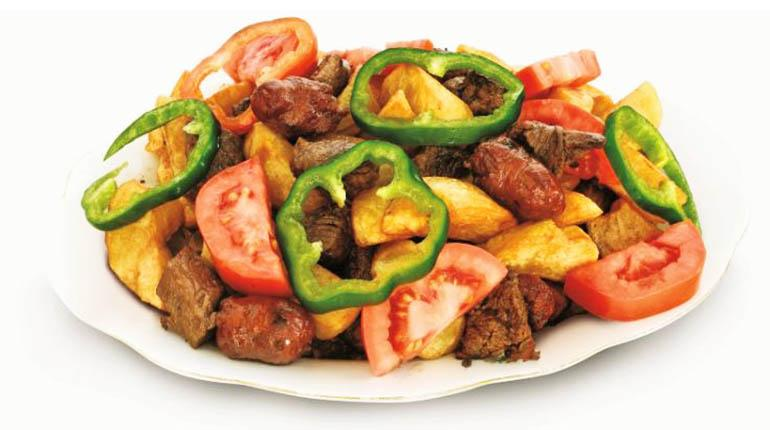
\includegraphics[scale=0.2]{pique_macho} 
        } & 
        \vspace{-1.5cm}
        \begin{compactitem} 
            \begin{footnotesize}
                \item 1 kilo de carne de res (lomo), picada en dados de 2\nicefrac{1}{2}cm.
                \item \nicefrac{1}{2} kilo de salchichas de calentar, picadas en rodajas o bastones
                \item 8 papas medianas
                \item 4 cebollas grandes picadas tipo pluma
                \item 2 tomates medianos
                \item 2 locotos picados en tiras o rodajas
                \item 1 cucharadita de pimienta molida
                \item 1 pisca de comino molido
                \item 2 cucharaditas de sal
                \item Ajo molido (opcional)
                \item 3 huevos cocidos picados en rodajas
                \item 1\nicefrac{1}{2} taza de aceite para freír
            \end{footnotesize}
        \end{compactitem}&
        \vspace{-1.5cm}
        1. Cortar la carne en dados pequeños y condimentarla con sal, ajo, pimienta y comino a gusto.
        2. Freír la carne tapando la cacerola para obtener una carne jugosa.
        3. Aparte, freír las salchichas cortadas en rodajas.
        4. Pelar y cortar las papas en bastones y freírlas en aceite caliente.
        5. Mezclar la carne, las papas fritas y las salchichas.
        6. Servir adornando con el locoto crudo picado en tiras largas, los huevos duros, la cebolla y el tomate. \\
        \hline
        
        %---JUEVES---%
        \pbox{20cm}
        {
            \rule{0pt}{3ex}\begin{large}\textbf{Jueves}\end{large}\\ 
            \rule{0pt}{2ex}Jak’a lawa \\
            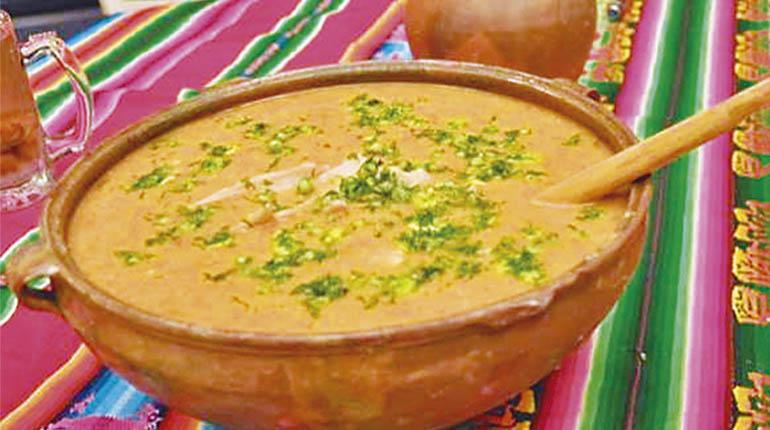
\includegraphics[scale=0.2]{jaka-lawa} 
        } & 
        \vspace{-1.5cm}
        \begin{compactitem} 
            \begin{footnotesize}
                \item \nicefrac{1}{2} kilo carne de res (cadera), cortada en seis porciones
                \item \nicefrac{1}{2} kilo de papas peladas, partidas en dos
                \item 5 litros de caldo
                \item 4 choclos grandes molidos en batán
                \item 2 cebollas peladas y picadas
                \item 5 dientes de ajo pelados y molidos
                \item 1 tomate pelado y picado
                \item 1 zanahoria pelada y rallada
                \item 1 nabo pequeño, pelado y rallado
                \item 1 achojcha picada en cuadraditos
                \item 2 ramitasde perejil picadas
                \item 2 vainas de ajíes rojo molidos
                \item \nicefrac{1}{4} cucharilla de comino molido
                \item 1 cucharilla de orégano desmenuzado
                \item \nicefrac{1}{2} taza de habas sin cascaras
                \item \nicefrac{1}{4} taza de arvejas sin cascara
                \item Aceite cantidad necesaria
                \item Sal a gusto
                \item 1 cuchara de perejil picado fino
                \item Queso raspado y perejil picado para servir
      \end{footnotesize}
        \end{compactitem}&
        \vspace{-1.5cm}
        1. Poner en una olla el agua al fuego, cuando empiece a hervir añadir la carne.
        2. Aparte, calentar el aceite en la sartén, sofreír la cebolla con el ajo hasta que doren, incorporar, el comino, el tomate, la zanahoria, el nabo, la achojcha, el perejil y el ají, mezclar y seguir cocinando.
        3. Vaciar en la olla donde se están cocinado las carnes el ahogado junto con las arvejas, dejar cocer 30 minutos.
        4. Añadir las papas, las habas, el choclo molido, el orégano y la sal, sin dejar de mover hasta que vuelva a hervir y estén cocidas las papas.
        5. Lo típico es servir en platos de barro (cerámica) con cucharas de palo (madera) echando encima perejil picado y queso rallado. \\
        \hline
        
        %---VIERNES---%
        \pbox{20cm}
        {
            \rule{0pt}{3ex}\begin{large}\textbf{Viernes}\end{large}\\ 
            \rule{0pt}{2ex}Llusp’ichi \\
            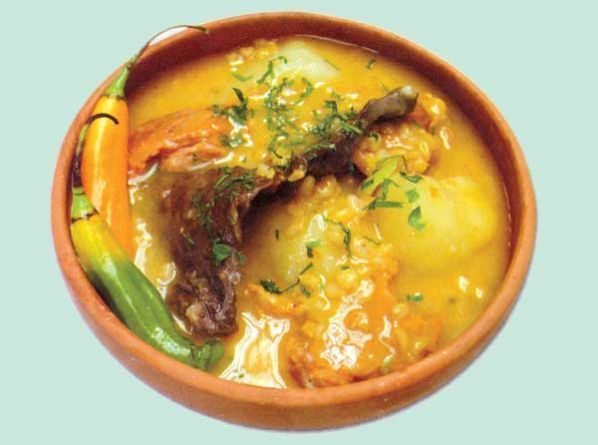
\includegraphics[scale=0.4]{lluspichi} 
        } & 
        \vspace{-2cm}
        \begin{compactitem} 
            \begin{footnotesize}
                \item \nicefrac{1}{2} kilo de trigo pelado
                \item \nicefrac{1}{2} kilo de papas peladas y partidas en dos
                \item \nicefrac{1}{2} kilo carne de cordero (nudos)
                \item \nicefrac{1}{4} kilo carne de res (cadera)
                \item Cuerito de cerdo un pedazo
                \item 2 cucharas de colorante rojo sin picante
                \item \nicefrac{1}{2} taza de habas sin cáscaras
                \item \nicefrac{1}{4} taza de arvejas sin cáscara
                \item 2 cebollas medianas picadas en cuadraditos
                \item 1 zanahoria pelada y rallada
                \item 1 nabo pequeño pelado y rallado
                \item 1 achojcha picada en cuadrados
                \item 2 ramitas de perejil picado
                \item 2 dientes de ajo pelados y molidos
                \item \nicefrac{1}{4} cucharilla de comino molido
                \item 4 cucharas de aceite
                \item 1 cuchara de orégano desmenuzado
                \item 6 litros de agua
                \item Sal a gusto
                \item 1 cuchara de perejil picado
            \end{footnotesize}
        \end{compactitem}&
        \vspace{-2cm}
        Remojar el trigo pelado noche antes. Al día siguiente lavar en varias aguas, retirando la tierra y piedrecillas.
        Poner al fuego una olla con el agua. Cuando empiece a hervir añadir las carnes de cordero, de res, el cuerillo de cerdo y el trigo.Aparte calentar el aceite en la sartén en el fuego y sofreír la cebolla con el ajo. Dejando dorar, incorporar el comino, el perejil, la achojcha, el nabo, la zanahoria, el colorante y las arvejas. Añadir este ahogado a la olla y dejar cocer. Mover continuamente para que no se pegue al fondo de la olla, hasta que las carnes estén suaves y el trigo reviente, luego incorporar las papas, las habas. Sazonar con la sal y el orégano, al final si está muy líquido añadir un poco de harina diluida en agua sin grumos. Dejar cocer las papas y retirar del fuego. Servir caliente, \\
        \hline
        
        %---SABADO---%
        \pbox{20cm}
        {
            \rule{0pt}{3ex}\begin{large}\textbf{Sabado}\end{large}\\ 
            \rule{0pt}{2ex}Sopa de papaliza \\
            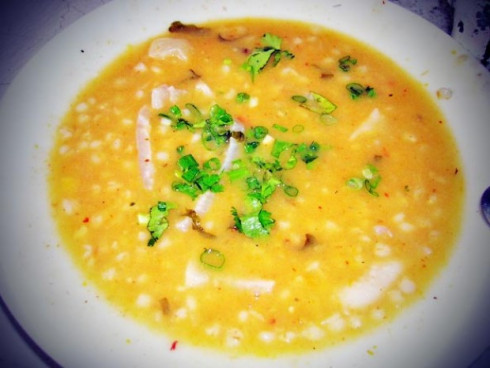
\includegraphics[scale=0.4]{sopa-de-papaliza} 
        } & 
        \vspace{-2cm}
        \begin{compactitem} 
            \begin{footnotesize}
                \item \nicefrac{1}{2} Kilo de costilla de res
                \item 1 Pedazo de chalona
                \item 3 Tazas de papalisa cocida y machucada
                \item 3 Cucharadas de aceite
                \item \nicefrac{1}{2} Taza de habas
                \item \nicefrac{1}{2} Taza de arvejas
                \item 1 Cebolla
                \item 2 Ramas de hierba buena
                \item 3 Papas
                \item Sal a gusto
                \item 2 Litros de agua
            \end{footnotesize}
        \end{compactitem}&
        \vspace{-2cm}
        Pon los dos litros de agua en una olla y hazla hervir.
Cuando este en plena ebullición agrégale la carne de res y la chalona. Déjalas cocer a fuego moderado.
En una sarten calienta un poco el aceite y refrié la papalisa, agrega las arvejas, las habas y la cebolla picada a la pluma.
Pon la papalisa en el caldo donde se esta cociendo la carne y déjala cocer muy bien. Desde que la papalisa este cocida agrega las papas peladas y el resto en el sarten.
Espera a que todo haya cocido muy bien para sazonar con sal y servir con hierba buena picada fina encima para adornar. \\
        \hline
    
    \newpage
    \end{tabular}
    \end{document}
